\begin{recipe}
    [% 
        preparationtime = {\unit[30]{min}},
        bakingtime = {\unit[30]{min}}
    ]
    {Sweet buns with curd cheese}
    \introduction{%
        Curd cheese is essential.
        It's high time for a trip to a Polish shop, if you haven't already done so.
        If there's big Polish diaspora  in the city, sometimes you can buy it in Tesco but don't confuse it with quark, it's something different (see introduction to a Polish shop for details).

        More fancy version involves raspberries or fresh apricots (halfs) and crumble topping
    }

    \ingredients[12]{%
        \unit[500]{g} & Flour \\
        \unit[40]{g} & Yeast fresh* \\
        2 tbs. & Sugar \\
        2 ts. & Sugar (leaven) \\
        1 c. & Milk \\
        2 & Eggs \\
        50 g. & Melted butter \\
        & \textbf{Filling} \\
        400 g & Curd cheese \\
        1 & Egg yolk \\
        \nicefrac{1}{2} c. & Sugar \\
        \unit[50]{g} & Butter, melted
    }

    \preparation{%
        \step Leaven: dissolve yeast in warm milk (heat milk so you can easily dip your finger in without burning yourself).
        Add 2 teaspoons of sugar and 1 of flour.
        Leave in dark cupboard for about 10 min.
        \underline{Watch out!} It grows, make sure there's enough room in mug/pot/bowl.

        \step Knead dough (start with flour, leaven and eggs, then add melted butter), cover with a cloth and leave in warm place (cupboard, room) for 30-60 min (the dough should almost double its size).

        \step In meantime, blend curd cheese with egg yolk, butter and sugar.
        It should be smooth and creamy.

        \step Form round, quite flat buns.
        Leave for 15 min to grow (cover with cloth).

        \step With the help of glass, form a valley in the middle and fill it with cheese.
        If using raspberries, add them now, on the cheese (press in cheese).

        \step \underline{Bake at \unit[180]{\textcelcius} for 20 min.}
        \vspace{2cm}
    }

    \suggestion
    {%
        For buns and bread I prefer to use fresh yeasts.
        Usually I buy them in Polish shop.
        Nevertheless, dried yeast should work too.
        My converter: 15g fresh $=$ 7g dried.

        If you use dried yeast, there's no need to do a leaven (in theory).
        I usually like to do it anyway.
    }

    \hint{%
        Bone of contention: Magda believes that when doing yeast dough,
        it shouldn't be in contact with metal surface (spoon, bowl etc) (apart for fork which is necessary to prepare leaven).
        I don't believe in such a thing, though.
    }

\end{recipe}

\begin{figure}[h]
    \centering
    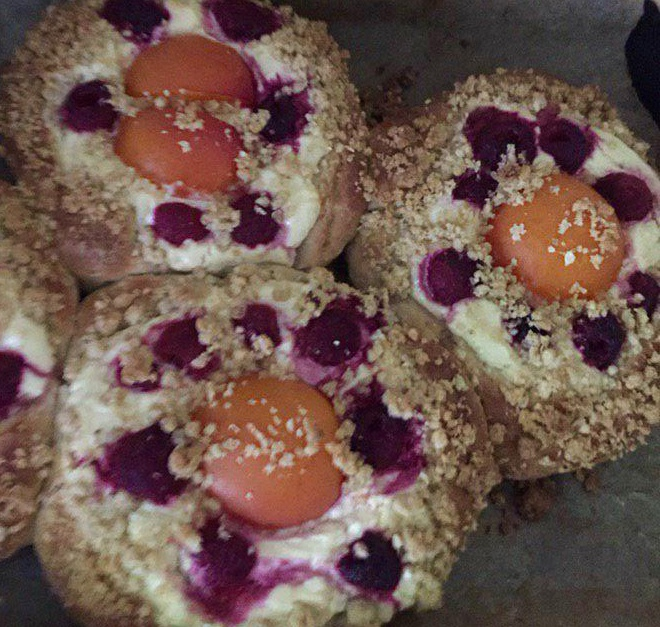
\includegraphics[width=8cm]{pic/buns_apricot_quark}
\end{figure}

\begin{figure}[h]
    \centering
    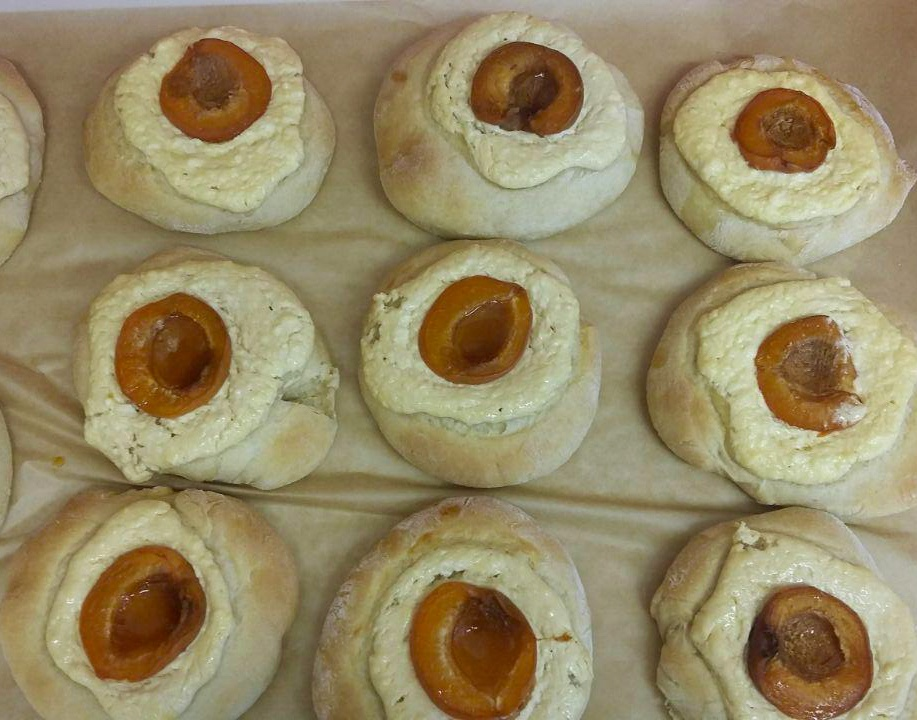
\includegraphics[width=8cm]{pic/buns_apricot}
\end{figure}
% TODO: alongside